% (The MIT License)
%
% Copyright (c) 2023 Yegor Bugayenko
%
% Permission is hereby granted, free of charge, to any person obtaining a copy
% of this software and associated documentation files (the 'Software'), to deal
% in the Software without restriction, including without limitation the rights
% to use, copy, modify, merge, publish, distribute, sublicense, and/or sell
% copies of the Software, and to permit persons to whom the Software is
% furnished to do so, subject to the following conditions:
%
% The above copyright notice and this permission notice shall be included in all
% copies or substantial portions of the Software.
%
% THE SOFTWARE IS PROVIDED 'AS IS', WITHOUT WARRANTY OF ANY KIND, EXPRESS OR
% IMPLIED, INCLUDING BUT NOT LIMITED TO THE WARRANTIES OF MERCHANTABILITY,
% FITNESS FOR A PARTICULAR PURPOSE AND NONINFRINGEMENT. IN NO EVENT SHALL THE
% AUTHORS OR COPYRIGHT HOLDERS BE LIABLE FOR ANY CLAIM, DAMAGES OR OTHER
% LIABILITY, WHETHER IN AN ACTION OF CONTRACT, TORT OR OTHERWISE, ARISING FROM,
% OUT OF OR IN CONNECTION WITH THE SOFTWARE OR THE USE OR OTHER DEALINGS IN THE
% SOFTWARE.

\documentclass{article}
\usepackage{../sqm}
\usepackage{amsmath}
\usepackage{relsize}
\newcommand*\thetitle{Source Code Volatility}
\begin{document}

\plush{\sqmTitlePage{12}}

\plush{
\pptBanner{Volatility Metric}
\begin{multicols}{2}
\scalebox{.7}{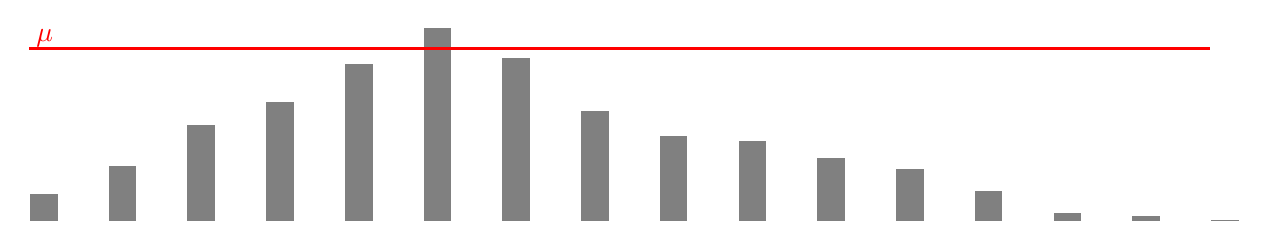
\begin{tikzpicture}[every node/.style={rectangle, minimum width=1em, fill=gray, anchor=south west, font={\color{white}}, inner sep=0pt}]
\node[minimum height=1em] at (0,0) {};
\node[minimum height=2em] at (1,0) {};
\node[minimum height=3.5em] at (2,0) {};
\node[minimum height=4.3em] at (3,0) {};
\node[minimum height=5.7em] at (4,0) {};
\node[minimum height=7em] at (5,0) {};
\node[minimum height=5.9em] at (6,0) {};
\node[minimum height=4em] at (7,0) {};
\node[minimum height=3.1em] at (8,0) {};
\node[minimum height=2.9em] at (9,0) {};
\node[minimum height=2.3em] at (10,0) {};
\node[minimum height=1.9em] at (11,0) {};
\node[minimum height=1.1em] at (12,0) {};
\node[minimum height=0.3em] at (13,0) {};
\node[minimum height=0.2em] at (14,0) {};
\node[minimum height=0.05em] at (15,0) {};
\draw[color=red, very thick] (0,2.2) node[fill=none] {\(\mu\)} -- (15,2.2);
\end{tikzpicture}}
\par
``The variance \(Var(g)\) is the \textbf{Volatility} of the source code.
The smaller the Volatility the more \textit{cohesive} is the repository
and the smaller the amount of the abandoned code inside it.''
\par\columnbreak\par
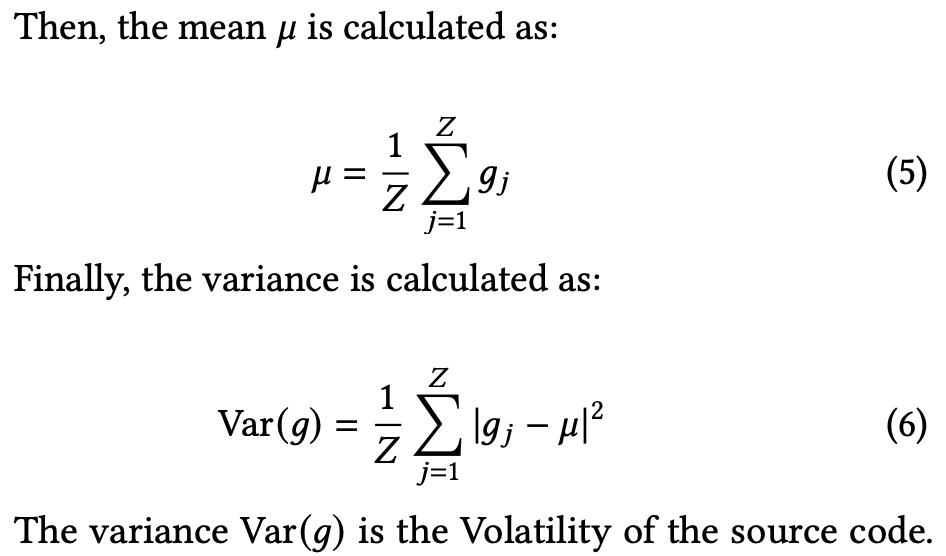
\includegraphics[width=.95\columnwidth]{formula.png}
\end{multicols}}

\plush{\pptBanner{Volatility vs. Number of Files in a Repo}\pptPic{.7}{graph.png}}

\pitch{\pptBanner{Monolithic Repositories}
{\small\begin{description}
\item[Centralization]
  The codebase is contained in a single repo encompassing multiple projects.
\item[Visibility]
  Code is viewable and searchable by all engineers in the organization.
\item[Synchronization:]
  The development process is trunk-based; engineers commit to the head of the repo.
\item[Completeness]
  Any project in the repo can be built only from dependencies also checked into the repo.
  Dependencies are unversioned; projects must use whatever version of their dependency is at the repo head.
\item[Standardization]
  A shared set of tooling governs how engineers interact with the code, including building, testing, browsing, and reviewing code.
\end{description}}\par
{\scriptsize Source: \textit{Advantages and Disadvantages of a Monolithic Repository: A case study at Google}, Ciera Jaspan et al., ICSE, 2018\par}}

\pitch{\pptQuote{ciera-jaspan.jpg}{Our survey results show that engineers at Google strongly prefer our monolithic repo, and that \emph{visibility} of the codebase and simple \emph{dependency management} were the primary factors for this preference.}{\textit{Advantages and Disadvantages of a Monolithic Repository: A case study at Google}, \emph{Ciera Jaspan}, Matthew Jorde, Andrea Knight, Caitlin Sadowski, Edward K. Smith, Collin Winter, Emerson Murphy-Hill, ICSE, 2018}}

\pitch{\pptQuote{matthew-jorde.jpg}{At Google, almost all code exists in a single large, central repo, in which almost all code is visible to almost all engineers. The repo is used by over 20,000 engineers and contains \emph{over 2 billion lines of code}.}{\textit{Advantages and Disadvantages of a Monolithic Repository: A case study at Google}, Ciera Jaspan, \emph{Matthew Jorde}, Andrea Knight, Caitlin Sadowski, Edward K. Smith, Collin Winter, Emerson Murphy-Hill, ICSE, 2018}}

\pitch{\pptQuote{durham-goode.jpg}{Facebook's main source repository is enormous–many times larger than even the Linux kernel, which checked in at \emph{17 million lines of code} and \emph{44,000 files} in 2013.}{\href{https://engineering.fb.com/2014/01/07/core-infra/scaling-mercurial-at-facebook/}{\textit{Scaling Mercurial at Facebook}}, Durham Goode et al., 2014}}

\pitch{\pptQuote{tomas-votruba.jpg}{Before monorepo, I had to upgrade every package manually, which resulted in dissonance: one package used Symfony\textbackslash{}Console 3.2, but other only 2.8 and it got messy \emph{for no reason}.}{\textit{How Monolithic Repository in Open Source saved my Laziness}, Tomas Votruba, 2017}}

\pitch{\pptBanner{Benefits of ``Manyrepo'' Approach}
{\small\begin{description}
\item[Encapsulation]
  Each repo encapsulates and hides its details from everybody else.
\item[Fast Builds]
  When a repo is small, the time its automated build takes is small.
\item[Accurate Metrics]
  Calculating LoC for a large repository doesn't make any sense.
\item[Homogeneous Tasks]
  It's easier to make tasks similar in size and complexity.
\item[Single Coding Standard]
  Smaller repositories look more beautiful.
\item[Short Names]
  Smaller namespaces mean better maintainability.
\item[Simple Tests]
  More dependencies are difficult to mock and test.
\end{description}}\par
{\scriptsize Source: \href{https://www.yegor256.com/2018/09/05/monolithic-repositories.html}{Monolithic Repos Are Evil} (2018)\par}}

\plush{
  \pptBanner{Read this:}\par
  \small
  \textit{Volatility Metric to Detect Anomalies in Source Code Repositories},
    Yegor Bugayenko,
    Proceedings of the 1st ACM SIGPLAN International Workshop on Beyond Code: No Code, 2021 \par
  \textit{Advantages and Disadvantages of a Monolithic Repository: A case study at Google},
    Ciera Jaspan, Matthew Jorde, Andrea Knight, Caitlin Sadowski, Edward K. Smith, Collin Winter, Emerson Murphy-Hill,
    Proceedings of the International Conference on Software Engineering, 2018 \par
  \href{https://www.yegor256.com/2018/09/05/monolithic-repositories.html}{Monolithic Repos Are Evil} (2018) \par
}

\end{document}
